

%----------------------------------------------------------------------------------------
%	PART
%----------------------------------------------------------------------------------------


\part{Capítulo cinco}
\graphicspath{ {img/ch5/}, {img/} }

%----------------------------------------------------------------------------------------
%	CHAPTER 5
%----------------------------------------------------------------------------------------

\chapterimage{ima2} % Chapter heading image


\chapter{Series uniformes diferidas, perpetuas y generales}
\section{Fórmulas del capítulo}

\begin{spacing}{1.5}
\begin{center}
\begin{tabular}{ |p{4cm}|p{7cm}| p{4cm}|}
\hline 
\rowcolor{orange!50}
\begin{center}\textbf{Fórmula}\end{center} & \begin{center}\textbf{Nombre}\end{center} & \begin{center} \textbf{Excel}\end{center} \\ \hline                        

$VP = \frac{R}{i}$ & Valor presente serie perpetua vencida & VA(i;n;R;0)\\ \hline 
 
\end{tabular}
\end{center}
\end{spacing}

\section{Series uniformes diferidas}
Las series uniformes vistas en el capítulo anterior eran inmediatas porque con el primer pago se encontraba el primer período, pero puede ser que el primer pago se encuentre después de haber pasado cierta cantidad de períodos, en este caso se denomina serie uniforme diferida, tal como se puede apreciar en el siguiente ejemplo: \\

\textbf{Ejemplo 1:}\\
Una  industria  vende  toda  su  producción  y  si  pudiera  producir  más  vendería  más, por  tal  motivo  le  ha  solicitado  al  banco  de  donde  él  es  cliente  que  le  presten  \$8 millones  para  ser  cancelado  en  20  pagos  trimestrales  de \$R c/u,  pero  también solicita  que le  permitan  efectuar  el  primer  pago  exactamente al  año  de  que  se le conceda  el  préstamo,  esta  solicitud  la  hace  debido  a  que  con  el  dinero  del  préstamo  va  a  comprar  en  el  exterior  la  maquinaria  necesaria  para  hacer  las ampliaciones en su fábrica, lo cual requiere del tiempo necesario para la importación, nacionalización, transporte, período de montaje y pruebas, hasta dejarla a punto para la producción. Calcular el valor de la cuota trimestral a cancelar, si le cobran una tasa de interés del 36\% nominal anual trimestre vencido (natv).\\

\textbf{Solución:}

\begin{itemize}
	\item a. Diagrama de flujo de caja:
	\begin{center}
		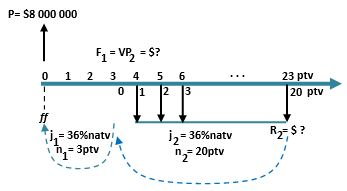
\includegraphics[height=4.0cm]{5_1}
	\end{center}
	Se establecerá la fecha focal en el período 0. La serie uniforme vencida debe comenzar en el período 3, el primer flujo de pago vencido en el período 4 y terminar en el período 23, equivalente a 20 pagos trimestrales vencidos efectuados. Se calcula el VP de la serie en n=3 ptv. La doble numeración no siempre es necesaria, aquí la hemos puesto para dar mayor claridad al ejemplo.\\
	
	\item b. Declaración de variables:
	\\VP = \$8'000.000\\
	$n_{1}$ = 3 ptv\\
	$n_{2}$ = 20 ptv\\
	j = 36\% natv\\
	
	$i= \frac{36\% \ natv}{4 \ ptv} = 9\%$ptv\\
	

	
	\item c. Declaración de fórmulas:\\
	$VP = R(\frac{1-(1+i)^{-n}}{i})$ Valor presente de una serie uniforme vencida\\
	$P= F{(1+i)}^{(-n)}$ Valor presente\\
	
	\item d. Procedimiento matemático:\\
	$\$8'000.000 = R\frac{1-(1+0,09)^{-20}}{0,09}*(1+0,09)^{-3}$ \hspace{35 pt} \textit{Valor Ecuación de valor}\\
	\item e. Respuesta\\
	R = \$1'134.926,20\\
\end{itemize}

\section{Series uniformes perpetuas}

Una serie uniforme que tiene infinito número de pagos se denomina serie uniforme vencida infinita o perpetua, en realidad, las series uniformes vencidas infinitas no existen, porque en este mundo todo tiene fin, pero, supondremos que una serie uniforme vencida es infinita cuando el número de pagos o ingresos es muy grande o cuando no se sabe cuántos pagos son, pero se sospecha que son muchos.\\

Este tipo de serie uniforme vencida se presenta, cuando se coloca un capital y únicamente se retiran los intereses.  Al deducir la fórmula de una serie uniforme vencida infinita debe tenerse en cuenta que solo existe el valor presente, porque el valor final de una serie uniforme vencida infinita sería infinito.\\

$ VP = \lim_{n\to \infty}R\frac{1-(1+i)^{-n}}{i} = \lim_{n\to \infty} R\frac{1-0}{i} = \frac{R}{i}$\\  	

VP = $\frac{R}{i}$ Valor presente de una serie uniforme vencida perpetua \\

\textbf{Ejemplo 2}\\

Hallar el valor presente de una renta perpetua vencida de \$10.000 mensuales, suponiendo un interés del 33\% nominal anual mes vencido (namv).\\

\textbf{Solución}\\
\begin{itemize}
    \item a. Diagrama de flujo de caja:\\
    \begin{center}
		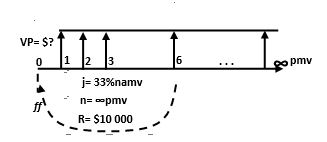
\includegraphics[height=4.0cm]{5_2}
	\end{center} 
	\item b. Declaración de variables\\
	R= \$10.000\\
	j= 33\% namv\\
	i = 2,75\% pmv\\
	n= $\infty$ \ pmv\\
	\item c. Declaración de fórmulas\\
	$VP = \frac{R}{i}$ Valor presente de una serie vencida perpetua\\
	\item d. Desarrollo matemático\\
	$VP = \frac{\$10\decimalpoint.000}{0,0275}$ = \$363.636,36 \hspace{35 pt} \textit{Ecuación de valor}\\
	\item e. Resultado\\
	El valor presente de la renta es \$363.636,36\\
\end{itemize}

\section{Series uniformes generales}

Las series uniformes vistas hasta el momento son aquellas en que el período de interés coincide con el período de pago. Todas ellas se denominan series uniformes simples.  Por  ejemplo:  una  serie  de  pagos  mensuales  con  una  tasa  periódica mensual  es  una  serie  uniforme  simple,  también  lo  sería  una  serie  de  pagos trimestrales con una tasa periódica trimestral, pero en el caso de una serie uniforme general es  cuando  el  período de  pago  no  coincide  con el período  de interés,  por ejemplo: si tenemos una serie de pagos trimestrales con una tasa periódica semestral o una serie de pagos mensuales con una tasa periódica anual (o una tasa nominal anual año vencido o una tasa Efectiva Anual, o tasa de referencia de la Superintendencia Financiera).\\

Una serie uniforme general puede ser reducida a una serie uniforme simple, si hacemos que los períodos de tiempo y los períodos de interés coincidan, hay dos formas para realizarlo:

La primera forma consiste en calcular pagos equivalentes que deben hacerse en concordancia con los períodos de interés.  Dicho en otras palabras, consiste en encontrar el valor de los pagos que, hechos al final de cada período de interés, sean equivalentes al pago único que se hace al final de un período de pago.\\

La segunda forma consiste en modificar la tasa, haciendo uso del concepto de tasas equivalentes, para hacer que coincidan los períodos de interés y de pago.\\

\textbf{Ejemplo 3:}\\
Hallar el valor futuro de una serie de 30 pagos trimestrales de \$25.000 c/u suponiendo una tasa del 24\% nominal anual mes vencido (namv). Use el procedimiento para modificar los pagos.\\

\textbf{Solución}\\
\begin{itemize}
	\item a. Diagrama de flujo de caja:
	\begin{center}
		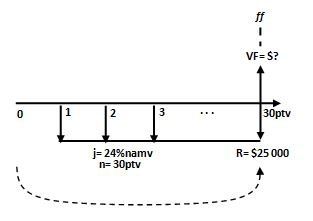
\includegraphics[height=4.0cm]{5_3_1}
	\end{center}
	La situación planteada en el problema es la siguiente:\\
	
	Para poder  solucionar  el  problema  tiene que coincidir el período de liquidación de intereses (el período del valor de j)con el período de liquidación de intereses (el periodo de n) y para llegar a esta coincidencia cambiaremos los pagos  de  trimestrales  a  mensuales,  entonces  un  pago  de  \$25.000  deberá  ser reemplazado por tres pagos mensuales de \$R que se calcularían así:\\ 
	
	\begin{center}
		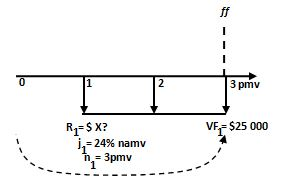
\includegraphics[height=4.0cm]{5_3_2}
	\end{center}
	
	
	\item b. Declaración de variables\\
    $i_{1}$ = 2\% pmv\\
    $n_{1}$= 3 pmv\\
	$VF_{1}$ = \$25.000\\
	$R_{1}$ = \$?\\
	
	\item c. Declaración de formulas\\
	VF = R$(\frac{(1+i)^n-1}{i})$ \hspace{35 pt} \textit{Valor futuro de una serie uniforme vencida}
	\\
	\item d. Desarrollo matemático\\
	Como el valor final de cada una de las gráficas debe ser igual, entonces:\\
	
	\$25.000 = R$\frac{(1+0,02)^3-1}{0,02} = \$X$ \hspace{35 pt} \textit{Ecuación de valor} \\
	R = \$8.168,87\\

	Esto significa  que  cada  pago  de  \$25.000  podrá  ser  reemplazado  por  tres  pagos mensuales de \$8.168,87 de manera que resultarán 90 pagos mensuales y la línea de tiempo que hemos dibujado inicialmente podrá ser reemplazada por:
	\begin{center}
		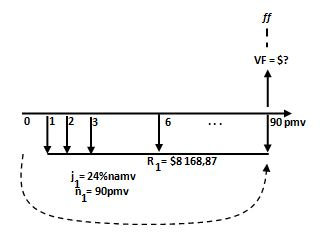
\includegraphics[height=4.5cm]{5_3_3}
	\end{center}

	\item e. Solución:\\
	VF = $\$8.168,87\frac{(1+0.02)^{90}-1}{0,02} = \$2.018,990$  \hspace{35 pt} \textit{Ecuación de valor}\\
\end{itemize}	

\textbf{Ejemplo 4:}\\
Resuelva el ejemplo anterior modificando la tasa.\\

\textbf{Solución}\\

Buscamos una i=?\% ptv equivalente al 24\% namv entonces:\\

\begin{itemize}
	\item a. Diagrama de flujo:\\
	\begin{center}
		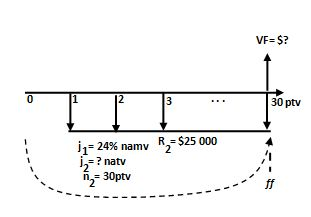
\includegraphics[height=5.5cm]{5_4_1}\\
	\end{center}
	
	
	\item b. Declaración de variables:\\
	$j_{1}$ = 24\% namv\\
	$i_{1}$ = 2\% pmv\\
	$m_{1}$ = 12 pmv \\
	$i_{2}$ = ?\% ptv\\
	$m_{2}$ = 4 ptv\\
	$j_{2}$ = ?\% natv\\
	n = 30 ptv\\
	 
	\item c. Declaración de fórmulas:\\
	
	$(1+i_{1})^{m_{1}} = (1+i_{2})^{m_{2}}$ Equivalencia de tasas\\
	$VF = R(\frac{(1+i)^n-1}{i})$ Valor futuro de una serie uniforme vencida\\
	
	
	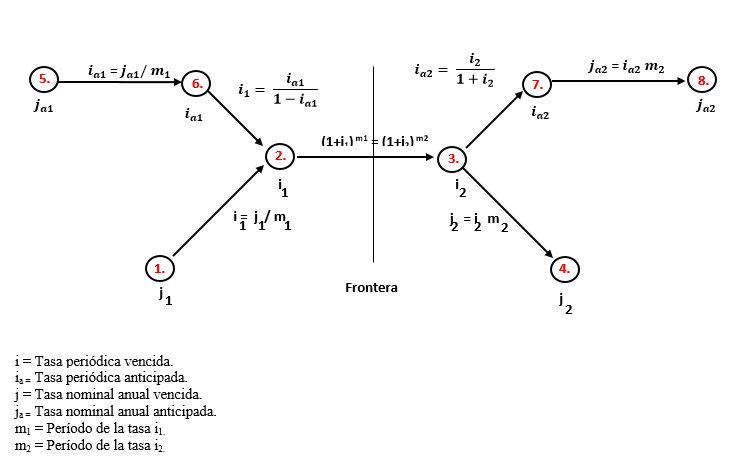
\includegraphics[height=8.5cm]{5_4_2}

	
	\item d. Procedimiento matemático:\\
	A partir del diagrama de equivalencia de tasas, se trata de recorrer del punto (1), $j_{1}$= 24\% namv al punto (4) $j_{2}$=?\% natv, pasando por los puntos (2) y (3).
	$(1+0,02)^{12} = (1+i)^4$\\
	
	i = 6,1208\% ptv\\
	
	VF = $\$25.000\frac{(1+0,061298)^{30}-1}{0,061208} = \$2.018,990$ \hspace{35 pt} \textit{Ecuación de valor}\\
	\item e. Respuesta\\
	VF = \$2.018,990\\
	Respuesta equivalente a la dada por el método de cambio de período de pagos trimestrales vencidos a mensuales vencidos.
\end{itemize}

\textbf{Ejemplo 5}\\
Una entidad estatal puede usar el edificio A, que requiere \$5 millones cada año como costo de mantenimiento y \$6 millones cada 5 años para reparaciones o, puede usar el edificio B, que requiere \$5.1 millones cada año como costo de funcionamiento y \$1 millón cada 2 años para reparaciones. Suponiendo una tasa del j=30\% nominal anual año vencido (naav) y que el edificio que se ocupe será por tiempo indefinido, ¿cuál de los dos edificios le resulta más conveniente utilizar?

\textbf{Solución:}\\
\begin{itemize}
	\item a. Diagrama de flujo de caja:\\
\\
	\textbf{Diagrama de flujo completo 	edificio A:}
	\begin{center}
		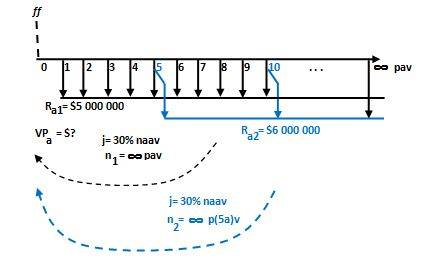
\includegraphics[height=5.9cm]{5_5_1}\\
	\end{center}
	\textbf{Diagrama de flujo desagregado en dos series	edificio A:}
		\begin{center}
		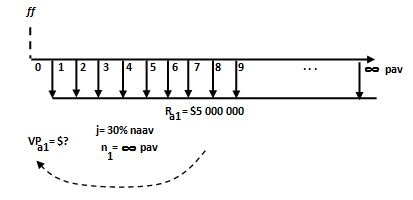
\includegraphics[height=5.5cm]{5_5_2}\\
	\end{center}
		\begin{center}
		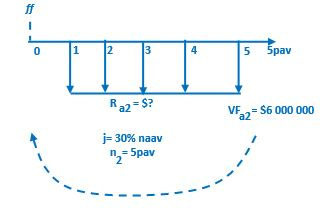
\includegraphics[height=5.5cm]{5_5_3}\\
	\end{center}
	\textbf{Diagrama de flujo completo edificio B:}
	\begin{center}
		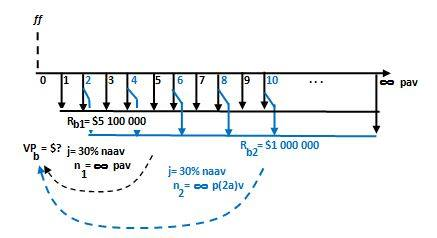
\includegraphics[height=6cm]{5_5_4}\\
	\end{center}
	\textbf{Diagrama de flujo desagregado en dos series	edificio B:}
		\begin{center}
		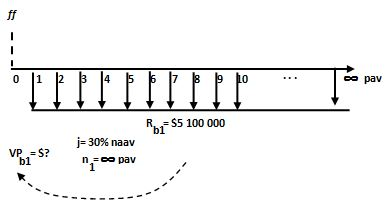
\includegraphics[height=5.5cm]{5_5_5}\\
	\end{center}
		\begin{center}
		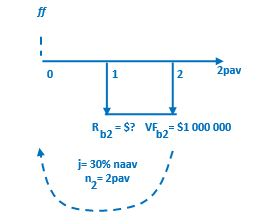
\includegraphics[height=5.5cm]{5_5_6}\\
	\end{center}
	
	Se calcula el valor presente para cada una de las series uniformes infinitas anuales de cada edificio. Para cada edificio se calcula la serie uniforme anual, producto de los egresos de reparaciones (\$6.000.000cada 5 años para el edificio A y \$1.000.000 para el edificio B). Luego se suman las series infinitas de mantenimiento y reparación para cada edificio y se comparan.
	
	\item b.Declaración de variables\\
	$R_{a1} = \$5'000\decimalpoint.000$ mante c/año $R_{a2} = \$6'000\decimalpoint.000$ repa c/5año\\
	$R_{b1} = \$5'100\decimalpoint.000$ mante c/año $R_{b2} = \$6'000\decimalpoint.000$ repa c/2año\\
	$R_{b2} = \$1'000\decimalpoint.000$ para reparación c/2año\\
	j = 30\% pav equivalente a i = 30\% naav\\
	$VP_{a} = \$?$ $\$VP_{b} = \$?$\\
	
	\item c. Declaración de fórmulas\\
	VF = $R(\frac{(1+i)^n-1}{i})$ Valor futuro de una serie uniforme vencida\\
	
	VP = $\frac{R}{i}$Valor presente de una serie perpetua vencida\\
	
	\item d. Procedimiento matemático\\
	Para el edificio A:\\
	Cálculo de la R anual equivalente de la serie quinquenal de reparación: \\
	$VF_{a2} = R_{a2}[\frac{(1+i)^n-1}{i}] => \$6'000\decimalpoint.000 = R_{a2}[\frac{(1+0,3)^5-1}{0,3}]$ \hspace{35 pt} \textit{Ecuación de valor}\\ \\
	$R_{a2} = \$663\decimalpoint.489,29$\\ \\
	Cálculo del valor presente de la serie uniforme vencida perpetua del costo anual de mantenimiento: \\
	$VP_{a1} = \frac{\$5'000\decimalpoint.000}{0,3} = \$16'666\decimalpoint.666,67$\\ \\
	Cálculo del valor presente de la serie uniforme vencida anual perpetua equivalente por la reparación: \\
	$VP_{a2} = \frac{\$663\decimalpoint.489}{0,3} = \$2'211\decimalpoint.630,97$\\ \\
	
	Suma de los valores presentes de las series uniformes vencidas anuales infinitas de mantenimiento y reparación:\\
	$VP_{a} = VP_{a1} + VP_{a2} = \$16'666\decimalpoint.666,67 + \$2'211\decimalpoint.630,97 = \$18'878\decimalpoint.797,69$\\
	
	Para el edificio B:\\
	Cálculo de la R anual equivalente de la serie bianual de reparación:\\
	$VF_{b2} = R_{b2}[\frac{(1+i)^n-1}{i}] => \$1'000\decimalpoint.000 = R_{b2}[\frac{(1+0,3)^2-1}{0,3}]$\hspace{35 pt} \textit{Ecuación de valor}\\ \\
	$R_{b2} =$ \$$434\decimalpoint.783$\\ \\
	Cálculo del valor presente de la serie uniforme vencida perpetua del costo anual de mantenimiento: \\
	$VP_{b1} = \frac{\$5'100\decimalpoint.000}{0,3} = \$17'000\decimalpoint.000$\\ \\
	Cálculo del valor presente de la serie uniforme vencida perpetua del costo anual de reparación:\\
	$VP_{b2} = $\$$434\decimalpoint.782,608/0,3 = $\$$1'449\decimalpoint.275,36$\\ \\
    Suma de los valores presentes de las series uniformes vencidas anuales infinitas de mantenimiento y reparación: \\
	$VP_{b} = VP_{b1} + VP_{b2} = $\$$17'000\decimalpoint.000 + $\$$1'449\decimalpoint.275,36 = $\$$18'449\decimalpoint.275,36$ \hspace{35 pt} \textit{Ecuación de valor}\\
	$VP_{a} -VP_{b} = $\$$18'878\decimalpoint.797,69 - $\$$18'449\decimalpoint.275,36 = $\$$429\decimalpoint.522,33$\\
	
	\item e. Respuesta:\\
	Es más conveniente usar el edificio B, que representa un ahorro de \$429.522
	
	
\end{itemize}



%----------------------------------------------------------------------------------------
%	PART
%----------------------------------------------------------------------------------------

%\part{Parte Dos}

%----------------------------------------------------------------------------------------
%	CHAPTER 3
%----------------------------------------------------------------------------------------

%\chapterimage{ima2} % Chapter heading image


%Anexos
%\chapter*{Anexos}
%\addcontentsline{toc}{chapter}{\textcolor{ocre}{Anexos}}




%----------------

%----------------------------------------------------------------------------------------
%	BIBLIOGRAPHY
%----------------------------------------------------------------------------------------

%\chapter*{Bibliografía}
%\addcontentsline{toc}{chapter}{\textcolor{ocre}{Bibliografía}}
%\section*{Books}
%\addcontentsline{toc}{section}{Books}
%\printbibliography[heading=bibempty,type=book]



%----------------------------------------------------------------------------------------
%	INDEX
%----------------------------------------------------------------------------------------

\cleardoublepage
\phantomsection
\setlength{\columnsep}{0.75cm}
\printindex

%----------------------------------------------------------------------------------------

